\section{Database Population}
The next stage of the project following downloading the historical Bitcoin Blockchain data and storing it in CSV files is to use this data to populate a Neo4J graph database. 

\subsection{Why Neo4J?}
Graph DB's provide efficient traversing of nodes; allowing million of connections to be traversed per second per core \cite{RefWorks:doc:5c98f0c6e4b00cbb4da393d8}. Scaling independently to the size of the data-set, a graph database is excellently suited for storing the vast, complex data-set constituting the Bitcoin Blockchain. Neo4J is an open-source, NoSQL graph-database providing ACID compliant transactions.

\subsection{Database Design}

\subsubsection{Data Nodes}
\begin{itemize}
    \item \texttt{BLOCK} : A Bitcoin block, unique id being the block hash. 
    \item \texttt{TRANSACTION} : A Bitcoin transaction, unique id the txid property.
    \item \texttt{OUTPUT} : A transaction output, unique id the txid property concatenated with the outputs index in the transaction.
    \item \texttt{COINBASE} : The special type of input that mints new bitcoin - has not been produced by a transaction. 
    \item \texttt{ADDRESS} : A Bitcoin public address, unique id the public address itself.
    \item \texttt{ENTITY }: A known entity as collected from walletexplorer.com in section \ref{section-entity-tagging}. 
\end{itemize}

\subsubsection{Relationships}
I created several types of relationships to exist between nodes in Neo4J. The relationships can be seen in a visual representation below in figure \ref{fig:neo4j-layout}.
\begin{itemize}
    \item \texttt{CHAINED\_FROM} Exists between two blocks; represents the relationship between a block and it's parent block. 
    \item \texttt{MINED\_IN} Exists beween a transaction and a block. Represents the relationship between a transaction and the block it was mined in. 
    \item \texttt{LOCKED\_TO} Exists between a transaction output and an address. Represents the relationship between an output, and who it can be spent by. 
    \item \texttt{INPUTS} Exists between a transaction output and a transaction. Describes the relationship between an output and the transaction it later funds. 
    \item \texttt{OUTPUTS} Exists between a transaction and a transaction output. Shows the relationship between a transaction and the new outputs it generates. 
    \item \texttt{COINBASE} Exists between a Coinbase node and a block. Represents the special type of input to a transaction which generates new bitcoin, and is associated with a block as it was the miners reward for successfully mining the block. 
    \item \texttt{HAS\_ENTITY} Exists between entities and the addresses they are known to control (see fig \ref{fig:neo4j-has-entity}).
\end{itemize}

\begin{figure}[h!]
  \centering
  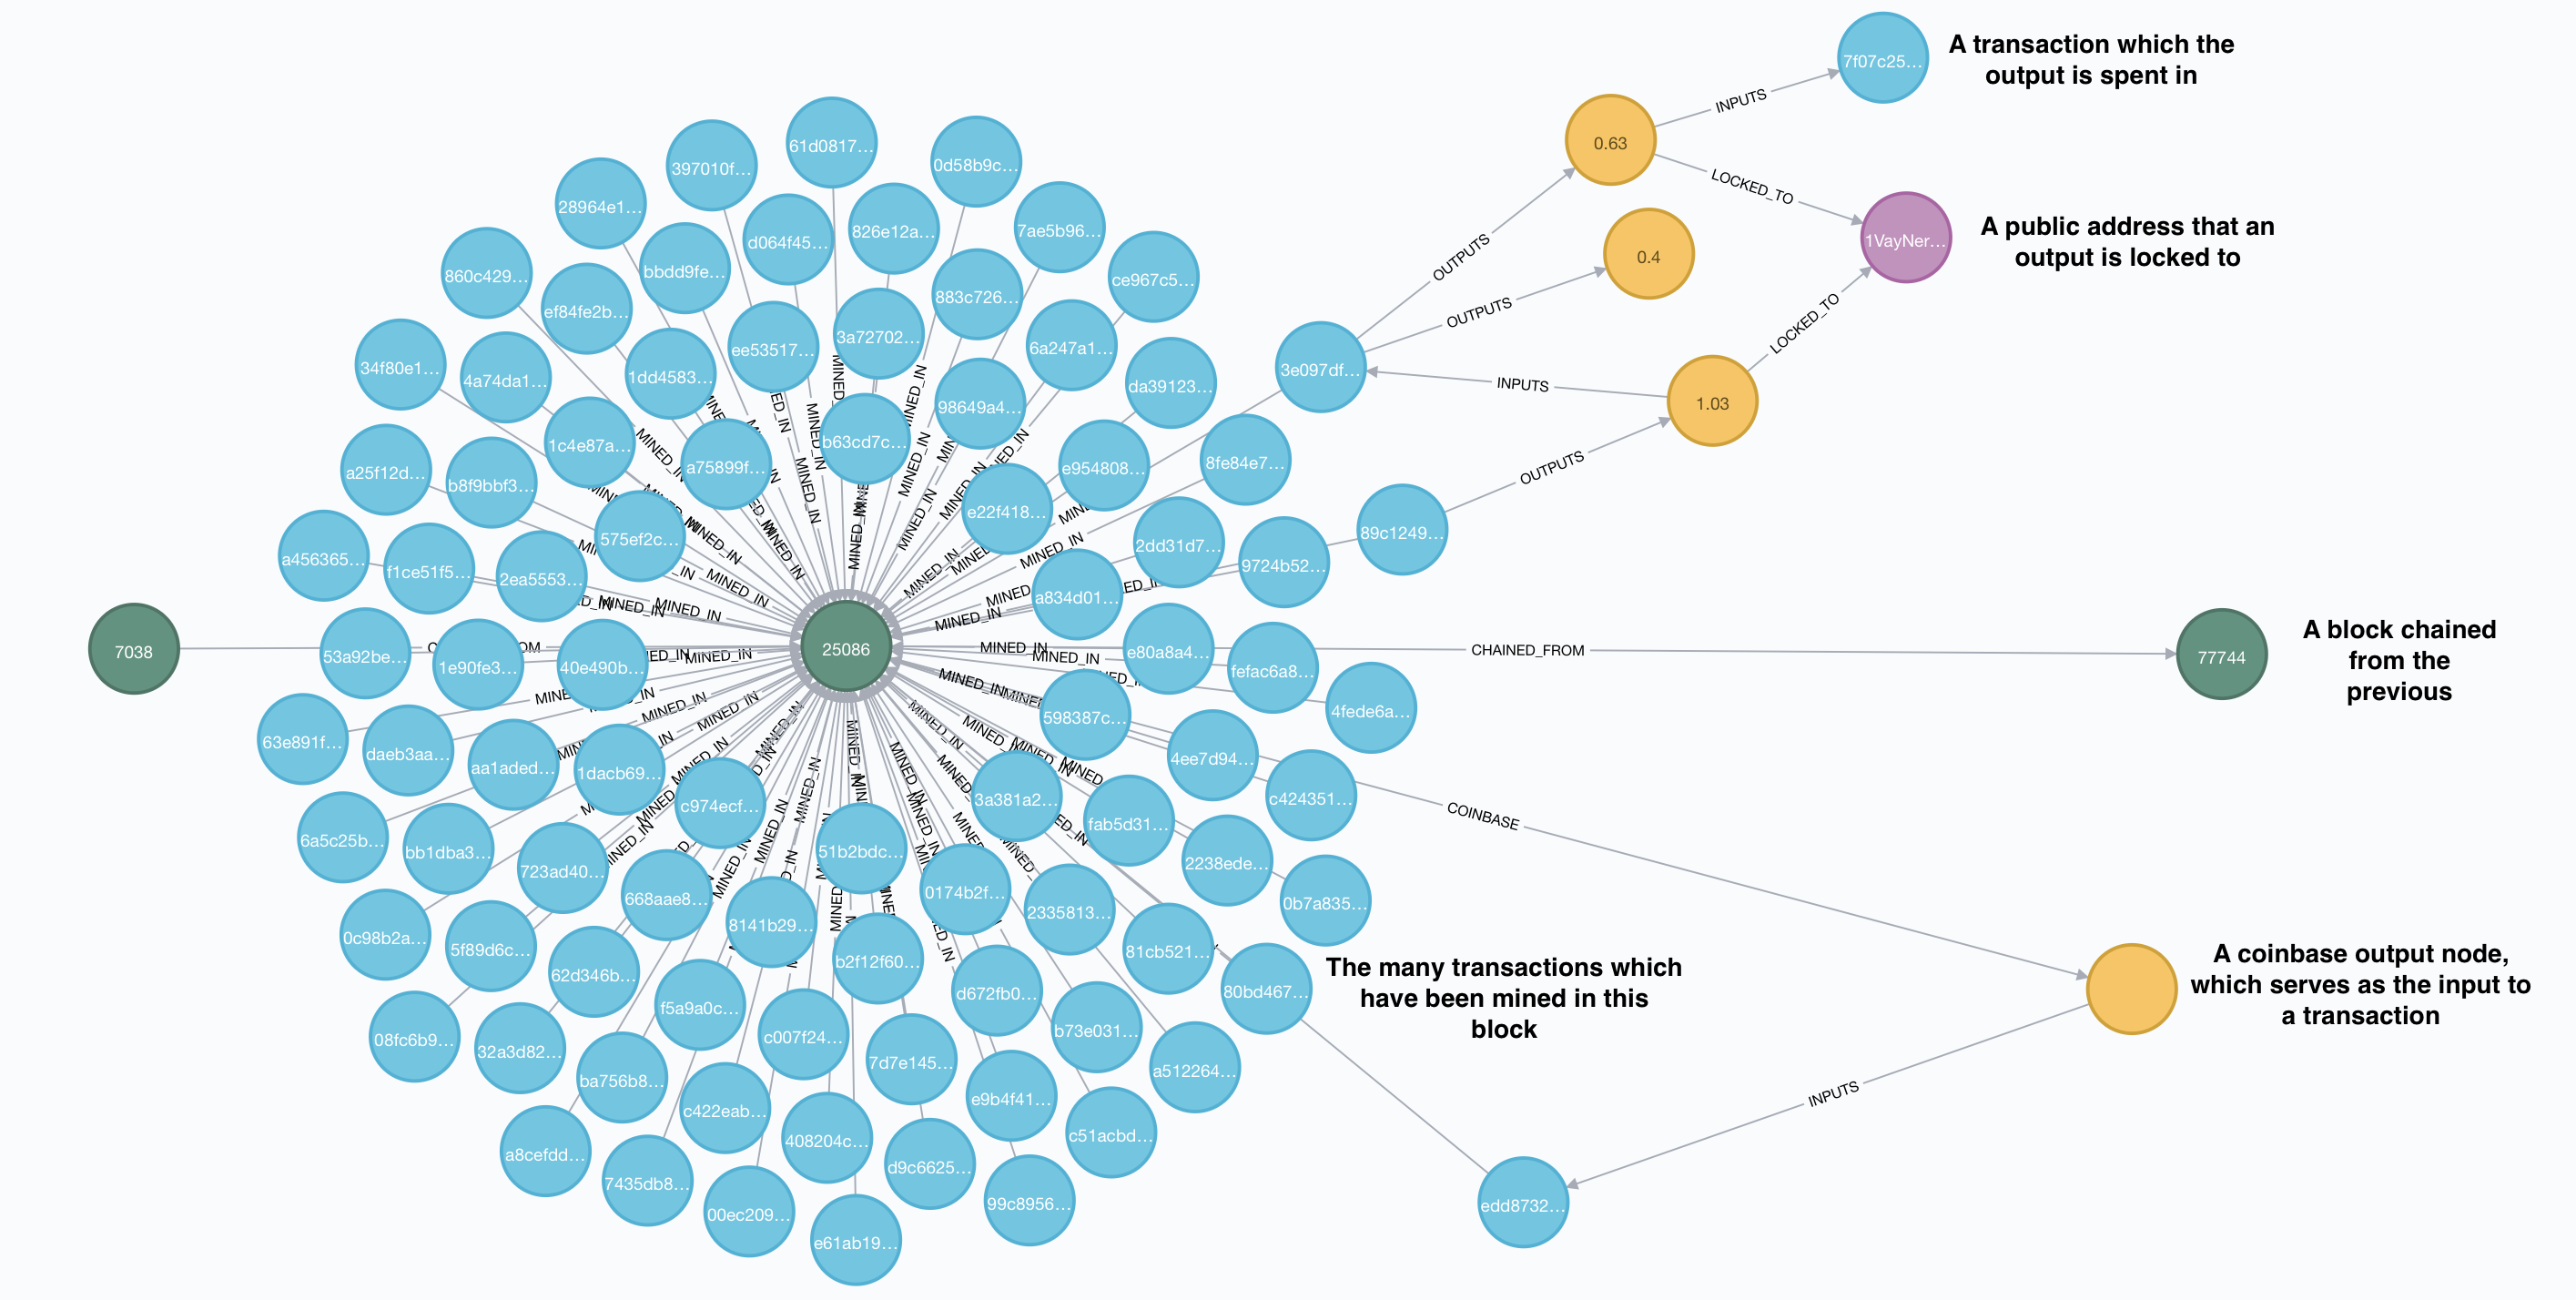
\includegraphics[width = 15cm]{./figures/neo4j-annotated}\\[0.5cm] 
  \caption{The nodes and relationships as visualised using the Neo4J Web UI}
  \label{fig:neo4j-layout}
\end{figure}

\begin{figure}[h!]
  \centering
  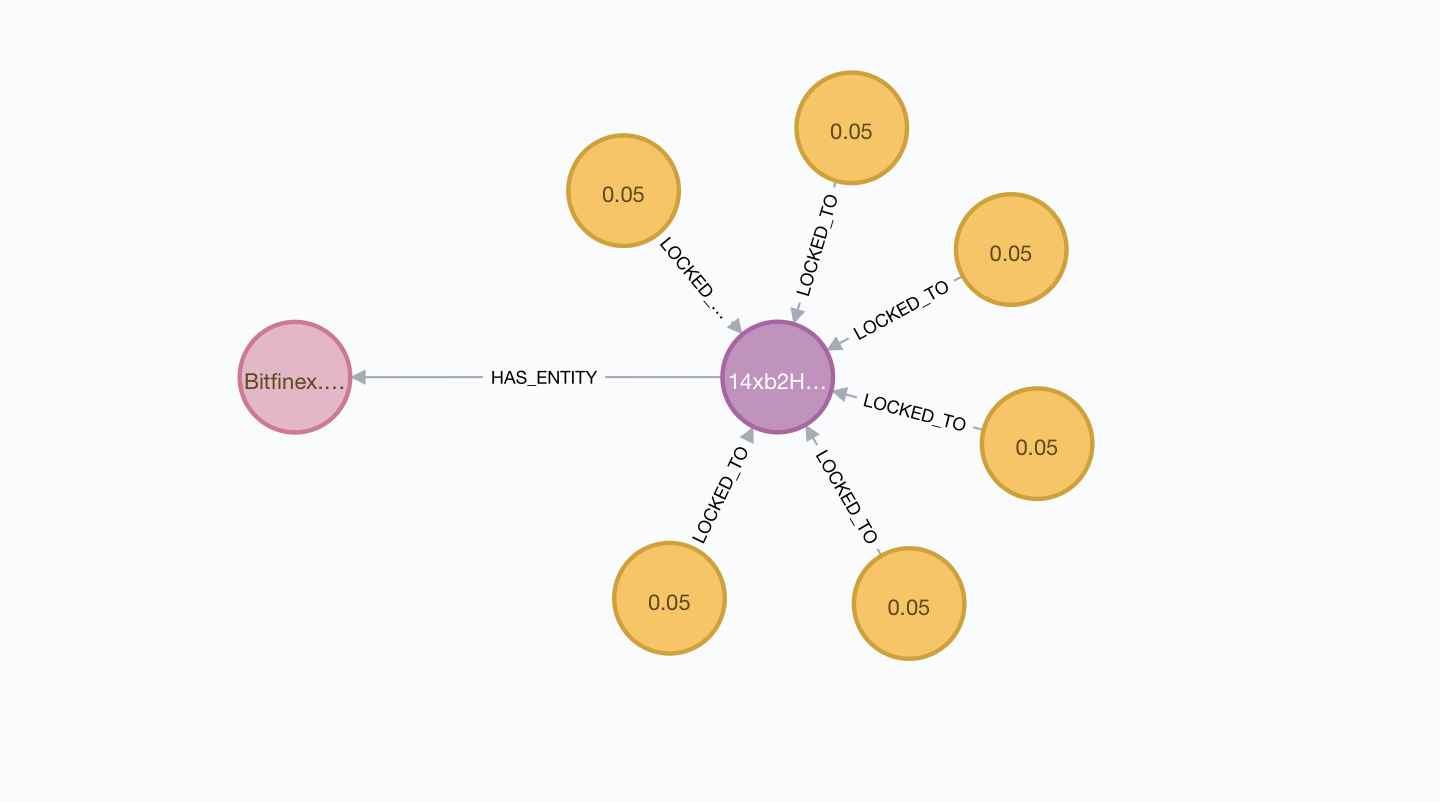
\includegraphics[width = 15cm]{./figures/has-entity-relationship}\\[0.5cm] 
  \caption{The new \texttt{HAS\_ENTITY} relationship visualised between a new Entity node and a bitcoin address.}
  \label{fig:neo4j-has-entity}
\end{figure}



\subsection{Invoking the import job}
I created a script to wrap the execution of the import job, providing the benefits of version control and reproducibility. This script first uses globbing to build the list of input files for each type of node and relationship. It then invokes the import command as shown below. Some additional arguments were \texttt{--max-memory} to override the default 90\% memory usage to use slightly more. The argument \texttt{--ignore-missing-nodes} was to prevent a long job failing simply due to a single relationship referring to a non existing node, and to rely on these bad relationships being reported to the file as defined by the \texttt{--report-file} option for manual investigation. 
\\\\
\begin{lstlisting}[language=Bash]
$1/bin/neo4j-admin import 
  --nodes:ADDRESS $address_files_all
  --nodes:BLOCK $block_files_all
  --nodes:COINBASE $coinbase_files_all
  --node:OUTPUT $output_files_all
  --nodes:TRANSACTION $transaction_files_all 
  --nodes:ENTITY $entity_files_all
  --relationships:CHAINED_FROM $relation_chained_from_files 
  --relationships:COINBASE $relation_coinbase_files 
  --relationships:INPUTS $relation_inputs_files 
  --relationships:LOCKED_TO $relation_locked_to_files 
  --relationships:MINED_IN $relation_mined_in_files 
  --relationships:OUTPUTS $relation_outputs_files 
  --max-memory 95% 
  --ignore-missing-nodes true 
  --report-file "neo4j-import-debug-report.log" 
\end{lstlisting}

\subsection{Challenges \& Solutions}
\subsubsection{Memory Issues}
While attempting to perform the bulk import, I encountered an issue where the import job would fail with no output other than message that the process was killed. This occurred deterministic at around 28\% progress into the graph node creation process. After investigation, I found that this issue was being caused by Neo4J running out of available memory; I rectified this by partitioning a much larger amount of Swap memory for the VM. The total amount of memory available (including swap) increased to over 30GB. This allowed the import tool to progress using swap once memory had been exhausted, albeit with increased memory access latency.

\subsubsection{Query Latency Issues} 
Upon successful population of the database, I performed simple entity lookups to begin to evaluate the correctness and performance of the database. However, I discovered immediately that simple searches for an address node using the tool takes an unacceptably long time (10 minutes 45 to find an Address node by its address and find its immediate neighbours). I used indexing to solve this issue. 

\subsubsection{Creating indexes}
Index's are useful for finding the starting point of a graph traversal. My tool requires exactly this functionality when we search for an address as the starting point of an investigation, before expanding out neighbours to traverse the blockchain. The initial search for the address is where the latency currently exists, therefore the first index I created was on the \texttt{address} property of the \texttt{ADDRESS} node. I was able to create this index by simply executing the command \texttt{CREATE INDEX ON :ADDRESS(address)} and using the command \texttt{CALL db.indexes} to track the progress of its population. 
\\\\
Once the index was created, the search for an address returned almost immediately. However, when trying to expand the relations of the address neighbours (non-address nodes) I encountered the same performance issues. I therefore had to create index's for the each node type using the unique ID that each node will be fetched with. The complete set of indexes created are:
\begin{itemize}
    \item \texttt{:ADDRESS(address)}
    \item \texttt{:BLOCK(hash)}
    \item \texttt{:ENTITY(name)}
    \item \texttt{:OUTPUT(outputId)}
    \item \texttt{:TRANSACTION(transactionId)}
\end{itemize}

\subsection{Import Result}
The import operation for the first 570,000 Bitcoin Blocks completed in 5 hours, 32 minutes and 54 seconds. The operation consumed 22.96GB of memory and created 1.964 billion nodes, 3.52 billion relationships and 3.03 billion properties. There were no errors or bad relationships reported. 